\chapter{\label{c:gw-detection}Gravitational waves}

\section{Event GW150914}
Around \num{1.3} billion years ago a pair of black holes, one with \num{36} solar masses and the other with \num{29} solar masses, merged into a single black hole with \num{62} solar masses \cite{Abbott2016}. The missing energy equivalent to \num{3} solar masses was radiated away in the form of gravitational waves.

At 09:50:45 \gls{UTC} on \nth{14} September 2015, gravitational waves from the event reached the \LIGO{} Livingston detector, perturbing the mirrors by \SI{e-18}{\meter} and creating a signal large enough for the electronics controlling the interferometer to detect the ripple in spacetime more than \num{23} times above the background noise. Seven milliseconds later, the same wavefront passed the \LIGO{} Hanford detector and moved the mirrors in the opposite direction. Meanwhile, computerised data analysis pipelines searching for coincident signals in each detector were running, and identified the event within a few minutes. Subsequent offline analysis using template banks representing waveforms produced by sources with different parameters were matched to the signal to calculate the most probable values. Given the significance of the signal above the detector's noise, and its fit to the templates, it was clear that the first detection of gravitational waves had been made.

The waveforms for event \emph{\GWFIRSTEVENT{}}, as it has become known, are consistent with a binary black hole merger in that they were swept up in frequency before creating a loud ``chirp'' signal as shown in Figure\,\ref{fig:gw150914}. The signal was only above each detector's background noise for the last few \SI{}{\milli\second} of this process, but it was consistent enough with theory that the collaboration could report a false alarm rate of less than \num{1} in \num{200000}. Not only did \LIGO{} make the first observation of a gravitational wave, it also made the first detection of a binary black hole system and found the missing experimental proof of Einstein's theory of general relativity. The field opening up due to \LIGO{} and the worldwide network of detectors in operation and under assembly, \GEO{}, \VIRGO{} and \KAGRA{}, represents an opportunity to study the universe in a completely new way.

\begin{figure}
  \centering
  \includegraphics[width=\columnwidth]{graphics/generated/from-python/10-gw150914.pdf}
  \caption[Measured strain from the LIGO Hanford and Livingston detectors around the time of event \GWFIRSTEVENT{}]{\label{fig:gw150914}Measured strain from the \LIGO{} Hanford and Livingston detectors around the time of event \GWFIRSTEVENT{}. Fast data pipelines work to find the best fitting template for the calibrated detector measurements from precomputed banks representing the various combinations of the system's parameters. Beyond this initial identification, computationally intensive analysis of the data around the time of the candidate event is processed using a variety of techniques to identify the most likely source parameters, and these can later be matched to numerical relativity models. The numerical relativity models best fitting the analysed data are shown for each site in the lower panel. These curves were originally presented in \cite{Abbott2016}, and they have been passed through a \num{35} to \SI{350}{\hertz} bandpass filter to remove higher and lower frequency background noise unrelated to the signals.}
\end{figure}
% data from https://losc.ligo.org/events/GW150914/
% Low frequency noise on the numerical relativity waveform is from the fact that the noise floor PSD of the detector is noisier than at high frequencies. This is probably because there is less data to FFT at lower frequencies by definition. So essentially it comes from the fact that the data was whitened first.

\section{Scientific outcomes from the first joint observation run}
The first detection was made shortly before a science run in which the two \LIGO{} detectors were kept at their most sensitive operating conditions as often as possible for a period of three months. In that time a second detection was made of a separate binary black hole merger, \GWSECONDEVENT{} \cite{Abbott2016b}, and taken alongside the first detection and another signal with lower significance it was possible for the \LSC{} and \VIRGO{} collaboration to make some important scientific discoveries. Among the outcomes from the observation run were that the first experimental tests of strong gravitational fields present during the events were still consistent with general relativity \cite{Abbott2016c}; that ``heavy'' black holes exist in nature and that they probably formed in an environment with low metallicity \cite{Abbott2016d}; and that the rate at which binary black holes merge in the known universe is constrained given the observations to between 9 and 240 per cubic gigaparsec per year \cite{lscvirgoo1}, suggesting that the advanced detectors might see dozens more in subsequent science runs.

Beyond the detection of binary black hole mergers, other sources such as compact neutron star binaries have yet to be found but are predicted to exist producing signals within the sensitivity of the detector networks for future science runs \cite{Abbott2016f}. Subsequent observations will hope to probe for new sources of gravitational waves, and with longer integration time it will be possible to set improved limits on the population of some of these astrophysical objects in our universe.

The long term goal of researchers in the field is to assemble a worldwide network of gravitational wave detectors to compliment the existing network of electromagnetic (\gls{EM}) telescopes to facilitate \emph{multi-messenger} astronomy. Such a network would be able to localise the sky position incident gravitational waves well enough to allow for \emph{\gls{EM} follow-up} \cite{Abbott2016e, Abbott2016f}, whereby the data from both telescopes and gravitational wave detectors can be combined to probe the astrophysics of the events in unprecedented detail and to identify and learn more about the nature and origin of host galaxies.

\section{General relativity and gravitational waves}
A consequence of Einstein's theory of general relativity, gravitational waves are produced by changes in the quadrupole moment of mass distributions such as the presence of non-spherical asymmetries in spinning objects or pairs of objects coalescing with elliptical orbits. The effect a gravitational wave has on spacetime as it propagates is to stretch it in one direction whilst contracting it in another. This \emph{strain} can be expressed as a linear combination of ``plus'' and ``cross'' polarisation terms, shown for an initially circular ring of test particles on a 2D plane as a function of phase angle in Figure\,\ref{fig:gravitational-wave-polarisation}.

\begin{figure}
  \centering
  \includegraphics[width=\columnwidth]{graphics/generated/from-svg/10-gravitational-wave-polarisation.pdf}
  \caption[Plus and cross polarisations of a propagating gravitational wave]{\label{fig:gravitational-wave-polarisation}Plus and cross polarisations of a propagating gravitational wave. As the wave travels, shown in this depiction perpendicularly to the plane of this page, it stretches spacetime in one direction while contracting it in the other in an elliptic behaviour. A gravitational wave can be described as a linear combination of the two polarisations.}
\end{figure}

Although in principle gravitational waves can be produced by all massive bodies, gravitational waves from Earth-bound objects, including the Earth itself, are not even remotely detectable. The strain in spacetime produced by such objects is so weak that there is no hope for us to make such a detection with any known technology. A good estimate for the strain produced by a pair of rotating objects is given as \cite{Sathyaprakash2009}:
\begin{equation}
  \label{eq:happrox}
  h \lesssim \frac{2 G \left( M v^{2} \right)_{\text{nonspherical}}}{c^4 r},
\end{equation}
where $G$ is the gravitational constant, $\left( M v^{2} \right)_{\text{nonspherical}}$ is the kinetic energy associated with the non-spherical parts of the source required for the creation of gravitational waves, $c$ is the speed of light and $r$ is the distance between the source and the detector. To get an idea of what the strain would be for man-made sources, we can consider as in \cite{Sathyaprakash2009} the case of two cars of mass $M = \SI{e3}{\kilo\gram}$ attached to opposite ends of a rod of length $d = \SI{10}{\meter}$, spinning about its centre in a centrifuge at a frequency of $f = \SI{10}{\hertz}$. The tangential velocity of the cars will be around $2 \pi f d \approx \SI{600}{\meter\per\second}$, about as fast as a modern fighter jet. Placing the detector one wavelength away, and using Equation\,\ref{eq:happrox}, the strain turns out to be around $\SI{4e-43}{}$. To be able to detect such a strain the current most sensitive detectors, \ALIGO{}, would require an improvement in sensitivity of \SI{20}{} orders of magnitude, which is clearly ludicrous.

A pair of solar-mass objects orbiting each other at \SI{100}{\hertz} within \SI{50}{\mega\lightyear} produces a strain of only one part in \SI{e21}{}, which is an amount only now detectable after decades of detector development. It is only the waves produced by the most violent redistribution of matter in the heaviest, most compact systems in the universe which we have any chance of detecting: binary black holes, compact binary neutron stars and core-collapse supernovae amongst others. Even then, gravitational radiation is only produced by the presence of a changing quadrupole moment and so only a subset of sources that happen to be in coalescence or contain surface asymmetries produce waves we have the ability to detect.

\section{Development of the gravitational wave detector}
Using the \emph{local Lorenz} gauge an incident gravitational wave can be described as a change in the distance separating two reference points in spacetime, and so a measurement of the length between pairs of test masses placed at the different points on the edges of the ellipses shown in Figure\,\ref{fig:gravitational-wave-polarisation} can be made to infer the presence of passing gravitational waves. Given the behaviour of the propagating waves, the primary degree of freedom they excite in such an apparatus is the differential mode of the distance separating the test masses, \LMINUS{}, which can be defined in terms of the position of the test masses $x_{\text{A}}$ and $x_{\text{B}}$ as:
\begin{equation}
  \label{eq:darm}
  \textrm{\LMINUS{}} = \frac{x_{\text{A}} - x_{\text{B}}}{2}.
\end{equation}
The strain of an incident gravitational wave, $h_0$, can be determined from the measured differential change in length between the test masses given the distance nominally separating the test masses, $L$:
\begin{equation}
  \label{eq:gw-strain}
  h_0 = \frac{\text{\LMINUS{}}}{L}.
\end{equation}

\subsection{Resonant bars}
The first attempts to detect gravitational waves began with Joseph Weber's studies in the 1960s with his \emph{Weber bar} \cite{Weber1960}. This was a device developed to act as a direct strain meter, with incident gravitational waves exciting the separation of the material along the length of the bar. Piezoelectric sensors placed on the surface of an aluminium cylinder convert changes in length into electrical signals. Whilst the expected change in length of such a cylinder from gravitational radiation would in most cases be tiny, the resonant frequency of the cylinder, typically in the kilohertz range, acts to enhance the amplitude of the length change at nearby frequencies. The sensitivity of such a bar as a function of frequency is determined in part by its quality factor (Q), with a necessary trade-off being made between peak sensitivity (high Q) and detection bandwidth (low Q). As sources of gravitational radiation are almost universally weak, the only reasonable hope of making such a detection is to choose a high Q material and hope for a favourable signal frequency.

Despite improvements over the following decades, the peak sensitivity of state-of-the-art resonant bar detectors was surpassed by \emph{interferometric} gravitational wave detectors in 2003 \cite{Pitkin2011} after it was shown that \emph{second generation} detectors improving upon the initial designs would offer superior sensitivity across a much wider bandwidth \cite{Harry2002a}. The interferometer was first suggested as a means for gravitational wave detection shortly after the introduction of the Weber bar \cite{Pustovoit1962}, but efforts to build prototypes and understand the significant sources of noise only gained momentum in the 1970s \cite{Moss1971, Weiss1972}.
% Gertsenshtein and Pustovoit contains: "We shall show below that this corresponds to a secondary effect, namely to resonant excitation of gravitational waves by the electromagnetic field." (p3)

\subsection{\label{sec:gw-interferometry}The gravitational wave interferometer}
The effect the strain shown in Equation\,\ref{eq:gw-strain} has on the round trip time $\tau$ measured by light travelling between two test masses is, taking for example the plus polarisation component $h_{+}$:
\begin{equation}
  \tau \approx \frac{2L}{c_0} - \frac{1}{2} \int^{t}_{t - \frac{2L}{c_0}} h_{+} \left( t \right) dt.
\end{equation}
Given that the speed of light, $c_0$, is constant, and the gravitational wave $h_0$ is a sinusoidal function with angular frequency $\omega_g$, this leads to a phase change $\delta \phi_{\text{GW}}$ as seen by the light with angular frequency $\omega_0$:
\begin{equation}
  \label{eq:gw-phase-change}
  \delta \phi_{\text{GW}} \left( t \right) \approx h_0 \frac{\omega_0}{\omega_g} \sin \left( \omega_g \frac{\tau}{2} \right) \cos \left( \omega_g \left(t - \frac{\tau}{2} \right) \right).
\end{equation}
This shows that the measurement of length between test masses with light offers the possibility to detect gravitational waves as phase fluctuations at the frequency of the signal. Gravitational wave induced phase modulation can also be described with the \emph{transverse traceless} gauge as a change in the refractive index of the space between fixed test masses. The effect is equivalent \cite{Saulson1997}, and so a change in length between the test masses can therefore be represented as a change in the frequency of the light, $\Delta \omega$, with respect to the light's nominal frequency:
\begin{equation}
  \label{eq:freq-to-length}
  h_0 = \frac{\text{\LMINUS{}}}{L} = \frac{\Delta \omega}{\omega_0}.
\end{equation}

From Equation\,\ref{eq:gw-phase-change} the \emph{modulation depth} (see Appendix\,\ref{sec:signal-sidebands}) can be approximated to $h_0 \frac{\omega_0}{\omega_g} \sin \left( \frac{\omega_g L}{c_0} \right)$, showing that, in principle, the longer the distance separating the test masses the more modulation an incident wave will impart to the light and the stronger the signal will be. This is true up until the point at which the sine wave is maximum, $\frac{\pi}{2}$ (or, as with the design of radio antennae, the point at which the length is one quarter of the incident wavelength), and so to be optimally sensitive to a \SI{100}{\hertz} gravitational wave the distance between the test masses must be around \SI{750}{\kilo\meter} which is clearly impractical for ground-based experiments. In Section\,\ref{sec:ifo-response} we will discuss techniques to avoid the need for such long baselines.
% Optimal frequency: omega_g * L / c_0 = \pi / 2, solve for L.

Figure\,\ref{fig:mi} shows the \MI{} topology that all current detectors are based on. Coherent light from a laser is incident at the input to a beam splitter whereupon it is coupled into two arms with highly reflective mirrors at each end. Perpendicular arms are most sensitive to the differential change in length in spacetime created by gravitational waves as shown in Figure\,\ref{fig:gravitational-wave-polarisation}. The light recombining at the beam splitter contains phase fluctuations from the motion of each test mass with respect to the beam splitter. If the arm lengths are arranged in such a way as to cancel the round-trip phase accumulation at the beam splitter in the absence of gravitational wave signal, the phase change between the arms due to a signal will appear at the beam splitter's \emph{output} port where it can be measured by a photodetector.

\begin{figure}
  \centering
  \includegraphics[width=0.5\columnwidth]{graphics/generated/from-svg/10-michelson.pdf}
  \caption[Simple \MI{}]{\label{fig:mi}The simple \MI{} used since the famous Michelson and Morley experiments of the 1880s.}
\end{figure}

Although this simple picture provides the foundation for the behaviour of the \MI{} as a gravitational wave detector, the operation of a real detector is more complex and requires its own discussion. Chapter\,\ref{c:instrumentation} will introduce the sensitivity improvements made to the \MI{} and the research into the main sources of noise affecting its sensitivity over the course of the last \num{40} years of development.

\section{Current and future interferometric detectors}
As of the time of writing the \ALIGO{} detectors in the USA are online and commissioners are working towards reaching the design sensitivity. \AVIRGO{}, situated in Italy, is due to begin science operations towards the end of 2016, with the \KAGRA{} detector in Japan due to follow in 2019\textemdash these are the \emph{second generation} detectors. \GEO{} in Germany has been operational in the years since the initial detectors stopped for upgrades, and is now transitioning into a detector-scale prototype facility. Planning is also under way to build an \ALIGO{} detector in India. The eventual network of detectors is shown in Figure\,\ref{fig:detector-network}\footnote{\INDIGO{}'s exact location is yet to be decided.}.

Beyond this generation, plans are afoot to build facilities which will push the sensitivity of the ground-based gravitational wave detector to the limit, with the so-called \emph{third generation} detectors. A European collaboration is working towards the \emph{\ET{}} \cite{ET2011} and the \LSC{} is working towards \emph{\LIGOCE{}} \cite{Dwyer2015, aligocosmic2016}. Efforts are also under way to complement these detectors with a space-based counterpart with significantly enhanced low frequency sensitivity, \emph{\ELISA{}} \cite{Amaro-Seoane2012}. Together, the network of ground- and space-based detectors will have unprecedented sensitivity from frequencies of \SI{}{\milli\hertz} to \SI{}{\kilo\hertz}, providing an ability to study the universe in unparalleled fidelity.

\begin{figure}
  \centering
  \includegraphics[width=\textwidth]{graphics/generated/from-python/10-detector-network.pdf}
  \caption[Worldwide interferometric gravitational wave detector network]{\label{fig:detector-network}Worldwide interferometric gravitational wave detector network. \GEO{}, \LHO{} and \LLO{} are operational, whilst \VIRGO{} and \KAGRA{} are being commissioned and \INDIGO{} is under construction. The locations of the \ET{} and \LIGOCE{} are as yet undecided.}
\end{figure}

\section{Thesis structure}
This thesis outlines work conducted with the goal of improving the sensitivity of future ground-based gravitational wave detectors.

Chapter\,\ref{c:instrumentation} introduces some theoretical foundations and motivation for the work presented in the rest of this thesis. Chapter\,\ref{c:waveguides} presents an investigation into \emph{waveguide} mirrors which offer a large potential improvement in Brownian thermal noise over conventional dielectric mirrors used in existing detectors. One downside is the potential presence of a coupling effect between transverse motion and reflection phase. This chapter presents an experiment conducted to measure this coupling in order to give a clearer picture of this mirror's potential use in future gravitational wave facilities.

The next set of chapters, \ref{c:speedmeter-intro}, \ref{c:speedmeter-control} and \ref{c:esd-concept}, present experimental research into a new type of gravitational wave interferometer: the \SSM{}. Chapter\,\ref{c:speedmeter-intro} introduces the concept in more detail and presents an overview of an ongoing proof-of-principle experiment taking place in Glasgow. Chapter\,\ref{c:speedmeter-control} highlights an important technical problem with the \SSM{} configuration which is not present with current detectors: that the controller cannot determine the displacement of the cavity mirrors at low frequencies, leading to loss of sensitivity. A solution to the problem is presented through the modelling of the complete control system using knowledge of the response and noise of the apparatus as well as estimates for noise in the experiment as fully assembled, backed by numerical simulations. Finally, Chapter\,\ref{c:esd-concept} outlines the architecture and construction of experimental apparatus to test a new actuator design to be used in the \SSMEXPT{}: a plate capacitor electrostatic drive. Designs and tests of a high-voltage amplifier to create the required test mass actuation are presented.

The main body of the work concludes with Chapter\,\ref{c:et-lf-control} where the current state of the sensing and control design for the low frequency interferometer as part of the planned Einstein Telescope facility is presented. This interferometer is to be primarily sensitive to frequencies below \SI{10}{\hertz} where existing detectors are dominated by seismic noise. Here, the sensing, controls and actuators found in the current generation of detectors are revisited through the use of numerical simulations.

Finally, the appendices provide additional information for the enthusiastic reader to support the main work. Appendix\,\ref{a:interferometry} provides a mathematical description of a basic interferometer and derives some useful figures of merit used throughout the work to describe interferometers. Appendix\,\ref{a:control} discusses some aspects of controls to complement the main text. Appendix\,\ref{a:simulation-tools} discusses the differences between the two main numerical simulation tools used for the presented work in Chapters \ref{c:speedmeter-intro}, \ref{c:speedmeter-control} and \ref{c:et-lf-control}. A conclusion is provided in Chapter\,\ref{c:conclusion}.